
\documentclass{beamer}
\mode<presentation>{
	\usetheme{Ilmenau}
	\usefonttheme{professionalfonts}
}
\usecolortheme{dolphin}
%Typical documenttypes: article/book
%some examples:
%\documentclass[reqno,11pt]{book}   %%%for books
%\documentclass[]{minimal}			%%%for Minimal Working Example






%%%%%%%%%%%%%%%%%%%% setting for fast compiling

%\special{dvipdfmx:config z 0}		% no compression

\includeonly{chapters/chapter9}		% In practice, use an empty document called "chapter9"	% usually for printing books






%%%%%%%%%%%%%%%%%%%% here we include packages

%%%basic packages for math articles
\usepackage{amssymb}
\usepackage{amsthm}
\usepackage{amsmath}
\usepackage{amsfonts}
\usepackage[shortlabels]{enumitem}	% It supersedes both enumerate and mdwlist. The package option shortlabels is included to configure the labels like in enumerate.

%%%packages for special symbols
\usepackage{pifont}					% Access to PostScript standard Symbol and Dingbats fonts
\usepackage{wasysym}				% additional characters
\usepackage{bm}						% bold fonts: \bm{...}
\usepackage{extarrows}				% may be replaced by tikz-cd
%\usepackage{unicode-math}			% unicode maths for math fonts, now I don't know how to include it

%%%basic packages for fancy electronic documents
%\usepackage[colorlinks]{hyperref}
%\usepackage[table,hyperref]{xcolor} 			% before tikz-cd. 
%\usepackage[table,hyperref,monochrome]{xcolor}	% disable colored output (black and white)

%%%packages for figures and tables (general setting)
\usepackage{float}				%Improved interface for floating objects
\usepackage{caption,subcaption}
\usepackage{adjustbox}			% for me it is usually used in tables 
\usepackage{stackengine}		%baseline changes

%%%packages for commutative diagrams
\usepackage{tikz-cd}
%\usepackage{quiver}			% see https://q.uiver.app/

%%%packages for pictures
\usepackage[width=0.5,tiewidth=0.7]{strands}
\usepackage{graphicx}			% Enhanced support for graphics

%%%packages for tables and general settings
\usepackage{array}
\usepackage{makecell}
\usepackage{multicol}
\usepackage{multirow}
\usepackage{diagbox}









 %https://tex.stackexchange.com/questions/58852/possible-incompatibility-with-enumitem










%%%%%%%%%%%%%%%%%%%% here we include theoremstyles

\numberwithin{equation}{section}

\theoremstyle{plain}
%\newtheorem{theorem}{Theorem}[section]

\newtheorem{setting}[theorem]{Setting}
%\newtheorem{definition}[theorem]{Definition}
%\newtheorem{lemma}[theorem]{Lemma}
\newtheorem{proposition}[theorem]{Proposition}
%\newtheorem{corollary}[theorem]{Corollary}
\newtheorem{conjecture}[theorem]{Conjecture}

\newtheorem{claim}[theorem]{Claim}
\newtheorem{eg}[theorem]{Example}
\newtheorem{ex}[theorem]{Exercise}
%\newtheorem{fact}[theorem]{Fact}
\newtheorem{ques}[theorem]{Question}
\newtheorem{warning}[theorem]{Warning}



\newtheorem*{bbox}{Black box}
\newtheorem*{notation}{Conventions and Notations}


\numberwithin{equation}{section}


\theoremstyle{remark}

\newtheorem{remark}[theorem]{Remark}
\newtheorem*{remarks}{Remarks}

%%% for important theorems
%\newtheoremstyle{theoremletter}{4mm}{1mm}{\itshape}{ }{\bfseries}{}{ }{}
%\theoremstyle{theoremletter}
%\newtheorem{theoremA}{Theorem}
%\renewcommand{\thetheoremA}{A}
%\newtheorem{theoremB}{Theorem}
%\renewcommand{\thetheoremB}{B}







%%%%%%%%%%%%%%%%%%%% here we declare some symbols

%%%%%%%DeclareMathOperator
%see here for why newcommand is better for DeclareMathOperator: https://tex.stackexchange.com/questions/67506/newcommand-vs-declaremathoperator

%%%%%basic symbols. Keep them!

%%%symbols for sets and maps
\DeclareMathOperator{\pt}{\operatorname{pt}}	%points. Other possibilities are \{pt\}, ...
\DeclareMathOperator{\Id}{\operatorname{Id}}	%identity in groups.
\DeclareMathOperator{\Img}{\operatorname{Im}}

\DeclareMathOperator{\Ob}{\operatorname{Ob}}
\DeclareMathOperator{\Mor}{\operatorname{Mor}}	%difference of Mor and Hom: Hom is usually for abelian categories
\DeclareMathOperator{\Hom}{\operatorname{Hom}}	\DeclareMathOperator{\End}{\operatorname{End}}
\DeclareMathOperator{\Aut}{\operatorname{Aut}}

%%%symbols for linear algebras and 
%%linear algebras
\DeclareMathOperator{\tr}{\operatorname{tr}}
\DeclareMathOperator{\diag}{\operatorname{diag}}	%for diagonal matrices

%%abstract algebras
\DeclareMathOperator{\ord}{\operatorname{ord}}
\DeclareMathOperator{\gr}{\operatorname{gr}}
\DeclareMathOperator{\Frac}{\operatorname{Frac}}

%%%symbols for basic geometries
\DeclareMathOperator{\vol}{\operatorname{vol}}	%volume
\DeclareMathOperator{\dist}{\operatorname{dist}}
\DeclareMathOperator{\supp}{\operatorname{supp}}

%%%symbols for category
%%names of categories
\DeclareMathOperator{\Mod}{\operatorname{Mod}}
\DeclareMathOperator{\Vect}{\operatorname{Vect}}
\DeclareMathOperator{\rep}{\operatorname{rep}} %usually rep means the category of finite dimensional representations, while Rep means the category of representations.
\DeclareMathOperator{\Rep}{\operatorname{Rep}}


%%%symbols for homological algebras
\DeclareMathOperator{\Tor}{\operatorname{Tor}}
\DeclareMathOperator{\Ext}{\operatorname{Ext}}
\DeclareMathOperator{\gldim}{\operatorname{gl.dim}}
\DeclareMathOperator{\projdim}{\operatorname{proj.dim}}
\DeclareMathOperator{\injdim}{\operatorname{inj.dim}}
\DeclareMathOperator{\rad}{\operatorname{rad}}


%%%symbols for algebraic groups
\DeclareMathOperator{\GL}{\operatorname{GL}}
\DeclareMathOperator{\SL}{\operatorname{SL}}

%%%symbols for typical varieties
\DeclareMathOperator{\Gr}{\operatorname{Gr}}
\DeclareMathOperator{\Flag}{\operatorname{Flag}}

%%%symbols for basic algebraic geometry
\DeclareMathOperator{\Spec}{\operatorname{Spec}}
\DeclareMathOperator{\Coh}{\operatorname{Coh}}
\newcommand{\Dcoh}{\mathcal{D}_{\operatorname{Coh}}}%%%This one shows the difference between \DeclareMathOperator and \newcommand
\DeclareMathOperator{\Pic}{\operatorname{Pic}}
\DeclareMathOperator{\Jac}{\operatorname{Jac}}

%%%%%advanced symbols. Choose the part you need!

%%%symbols for algebraic representation theory
\DeclareMathOperator{\Irr}{\operatorname{Irr}}
\DeclareMathOperator{\ind}{\operatorname{ind}}	%\ind(Q) means the set of  equivalence classes of finite dimensional indecomposable representations
\DeclareMathOperator{\Res}{\operatorname{Res}}
\DeclareMathOperator{\Ind}{\operatorname{Ind}}
\DeclareMathOperator{\cInd}{\operatorname{c-Ind}}


%%%symbols for algebraic topology
\DeclareMathOperator{\EGG}{\operatorname{E}\!}
\DeclareMathOperator{\BGG}{\operatorname{B}\!}

\DeclareMathOperator{\chern}{\operatorname{ch}^{*}}
\DeclareMathOperator{\Td}{\operatorname{Td}}
\DeclareMathOperator{\AS}{\operatorname{AS}}	%Atiyah--Segal completion theorem 

%%%symbols for Auslander--Reiten theory 
\DeclareMathOperator{\Modup}{\overline{\operatorname{mod}}}
\DeclareMathOperator{\Moddown}{\underline{\operatorname{mod}}}
\DeclareMathOperator{\Homup}{\overline{\operatorname{Hom}}}
\DeclareMathOperator{\Homdown}{\underline{\operatorname{Hom}}}


%%%symbols for operad
\DeclareMathOperator{\Com}{\operatorname{\mathcal{C}om}}
\DeclareMathOperator{\Ass}{\operatorname{\mathcal{A}ss}}
\DeclareMathOperator{\Lie}{\operatorname{\mathcal{L}ie}}
\DeclareMathOperator{\calEnd}{\operatorname{\mathcal{E}nd}} %cal=\mathcal


%%%%%personal symbols. Use at your own risk!

%%%symbols only for master thesis
\DeclareMathOperator{\ptt}{\operatorname{par}}	%the partition map
\DeclareMathOperator{\str}{\operatorname{str}}	%strict case
\DeclareMathOperator{\RRep}{\widetilde{\operatorname{Rep}}}
\DeclareMathOperator{\Rpt}{\operatorname{R}}
\DeclareMathOperator{\Rptc}{\operatorname{\mathcal{R}}}
\DeclareMathOperator{\Spt}{\operatorname{S}}
\DeclareMathOperator{\Sptc}{\operatorname{\mathcal{S}}}
\DeclareMathOperator{\Kcurl}{\operatorname{\mathcal{K}}}
\DeclareMathOperator{\Hcurl}{\operatorname{\mathcal{H}}}
\DeclareMathOperator{\eu}{\operatorname{eu}}
\DeclareMathOperator{\Eu}{\operatorname{Eu}}
\DeclareMathOperator{\dimv}{\operatorname{\underline{\mathbf{dim}}}}
\DeclareMathOperator{\St}{\mathcal{Z}}

%%%%%symbols which haven't been classified. Add your own math operators here!


\DeclareMathOperator{\Modr}{\operatorname{-Mod}}
\DeclareMathOperator{\BM}{\operatorname{BM}}




%%%%%%%newcommand

%%%basic symbols
\newcommand{\norm}[1]{\Vert{#1}\Vert}

%%%symbols only for master thesis
\newcommand{\dimvec}[1]{\mathbf{#1}}
\newcommand{\abdimvec}[1]{|\dimvec{#1}|}
\newcommand{\ftdimvec}[1]{\underline{\dimvec{#1}}}

\newcommand{\absgp}[1]{\mathbb{#1}}
\newcommand{\WWd}{\absgp{W}_{\abdimvec{d}}}
\newcommand{\Wd}{W_{\dimvec{d}}}
\newcommand{\MinWd}{\operatorname{Min}(\absgp{W}_{\abdimvec{d}},W_{\dimvec{d}})}
\newcommand{\Compd}{\operatorname{Comp}_{\dimvec{d}}}
\newcommand{\Shuffled}{\operatorname{Shuffle}_{\dimvec{d}}}

\newcommand{\Omcell}{\Omega}
\newcommand{\OOmcell}{\boldsymbol{\Omega}}
\newcommand{\Vcell}{\mathcal{V}}
\newcommand{\VVcell}{\boldsymbol{\mathcal{V}}}
\newcommand{\Ocell}{\mathcal{O}}
\newcommand{\OOcell}{\boldsymbol{\mathcal{O}}}
\newcommand{\preimage}[1]{\widetilde{#1}}
\newcommand{\orde}{\operatorname{ord}_e}
\newcommand{\fakestar}{*}

%as the subscription of Hom
\newcommand{\Alggp}{\text{-Alg gp}}







%%%%%%%%%%%%%%%%%%%% here we make some blocks for special features. 

%%%% todo notes %%%%
\usepackage[colorinlistoftodos,textsize=footnotesize]{todonotes}
\setlength{\marginparwidth}{2.5cm}
\newcommand{\leftnote}[1]{\reversemarginpar\marginnote{\footnotesize #1}}
\newcommand{\rightnote}[1]{\normalmarginpar\marginnote{\footnotesize #1}\reversemarginpar}









%%%%%%%%%%%%%%%%%%%% here we make some global settings. Understand everything here before you make a document!

%\usepackage[a4paper,left=3cm,right=3cm,bottom=4cm]{geometry}
%\usepackage{indentfirst}	% Indent first paragraph after section header

\setcounter{tocdepth}{2}


%https://latexref.xyz/_005cparindent-_0026-_005cparskip.html
\setlength{\parindent}{15pt}	
\setlength{\parskip}{0pt plus1pt}

%\setlength\intextsep{0cm}
%\setlength\textfloatsep{0cm}
\def\arraystretch{1}
%\setcounter{secnumdepth}{3}

\allowdisplaybreaks

% 设置图形文件的搜索路径
\graphicspath{{../figures/}}

\usepackage[T1]{fontenc}
\begin{document}

% The beginning depends on the documentclass. Rewrite this part if you use different documentclass!


\title{Geometry of Quiver Flag Varieties}
\author[Xiaoxiang Zhou]{Xiaoxiang Zhou\\[10mm]{\small Advisor: Prof. Dr. Catharina Stroppel \\ Second Advisor: Dr. Jens Niklas Eberhardt}}
\institute[Bonn uni]{Universität Bonn}
\date{\today}

\begin{frame}
	\titlepage
\end{frame}

\begin{frame}[fragile]{Introduction}
\begingroup
\def\arraystretch{1.2}
\begin{table}[]
\begin{tabular}{c|c|c|c}
\hline
Year & People             & Cohomology theory  & Algebra                                    \\ \hline
1980 & Kazhdan--Lusztig   & $\mathbb{C}[W]$    & $H_*^{\BM}(\St)$                           \\ \hline
1985 & Lusztig            & $\mathcal{H}_q(W)$ & $K^{G \times \mathbb{C}^{\times}} (\St)$   \\ \hline
2011 & Varagnolo-Vasserot & KLR algebra        & $H_{G_{\dimvec{d}}}^{*}(\St_{\dimvec{d}})$ \\ \hline
\end{tabular}
\end{table}
\endgroup

In the first part, we compute the $G$-equivariant $K$-theory of the Steinberg variety in the quiver version.
\end{frame}

\begin{frame}[fragile]{Variety structure}
	\begin{figure}[ht]
	\centering
		\vspace{0cm}
			\parbox[t]{.48\textwidth}{\centering
			\vspace{0cm}
			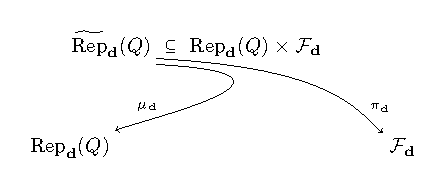
\includegraphics[width=5cm]{comm_diagram/incidence_variety_2.pdf}
			}
			\parbox[t]{.48\textwidth}{\centering
			\vspace{0cm}
			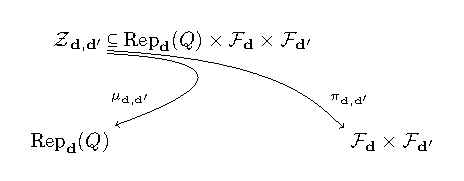
\includegraphics[width=5cm]{comm_diagram/incidence_variety_4.pdf}
			}
			\vspace{-7mm}
	\end{figure}
\end{frame}

\begin{frame}[fragile]{Stratification structure}
内容...
\end{frame}

\begin{frame}[fragile]{Main theorem}
\begin{theorem}
Under the convolution product, $K^{G_{\dimvec{d}}}(\St_{\dimvec{d}})$ has a $\Rpt(T_{\dimvec{d}})$-algebra structure. Moreover,
\begingroup
\upshape
\newcommand\labelenumi{(\theenumi)}
\begin{enumerate}
\item As an $\Rpt(T_{\dimvec{d}})$-module, $K^{G_{\dimvec{d}}}(\St_{\dimvec{d}})$ is free of rank $\abdimvec{d}!$;\label{item:A1}
\item As an $\Rpt(T_{\dimvec{d}})$-algebra, we can write down generators and relations explicitly.\label{item:A5}
\end{enumerate}
\endgroup 
\end{theorem}
For proving \eqref{item:A5}, we mainly use the localization formula and the excess intersection formula.
\end{frame}

\begin{frame}[fragile]{Generators}
$\begin{tikzcd}[ampersand replacement=\&]
	\textcolor{red}{\bullet} \& \textcolor{blue}{\bullet} 
	\arrow[from=1-1, to=1-2]
 \end{tikzcd}$, 
$\dimvec{d}=(3,2)$, 
$\MinWd =\left\{ ,\ldots \right\}$
\begin{figure}[ht]
  \vspace{0cm}
    \centering  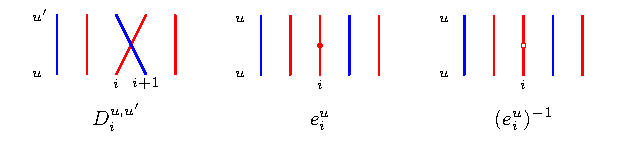
\includegraphics[width=8cm]{strands/generators.pdf}
      \label{fig:generators}        
\end{figure}
A typical element in $K^{G_{\dimvec{d}}}(\St_{\dimvec{d}})$ is a $\mathbb{Z}$-linear combination of diagrams shown below:
\begin{figure}[ht]
  \vspace{0cm}
    \centering  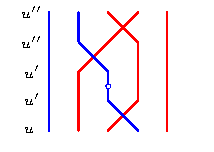
\includegraphics[width=3cm]{strands/glue_vertically_part.pdf}
      \label{fig:glue_vertically_part}        
\end{figure}
\end{frame}

\begin{frame}[fragile]{Compositions and trivial relations}
\begin{figure}[ht]
  \vspace{0cm}
    \centering  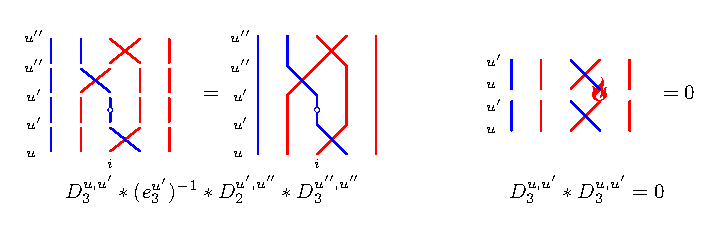
\includegraphics[width=7cm]{strands/glue_vertically.pdf}
      \label{fig:glue_vertically}        
\end{figure}

\begin{figure}[ht]
  \vspace{0cm}
    \centering  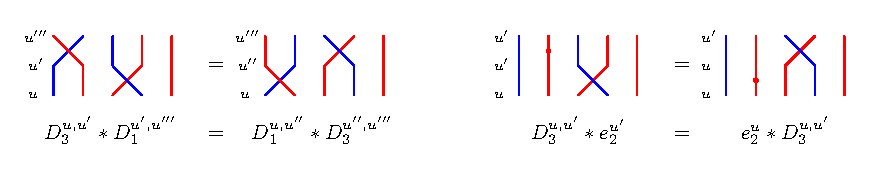
\includegraphics[width=10cm]{strands/clear_relations.pdf}
      \label{fig:clear_relations}        
\end{figure}
\end{frame}

\begin{frame}[fragile]{Nontrivial relations I}
\tikz[remember picture, overlay] \node[xshift=12mm, yshift=-2cm, anchor=west] at (current page.north west) {Same color: ($D_i^{u,u} \operatorname{\hat{=}} D_i, e_i^{u} \operatorname{\hat{=}} e_i$)};

\begin{figure}[ht]
  \vspace{0cm}
    \centering 
    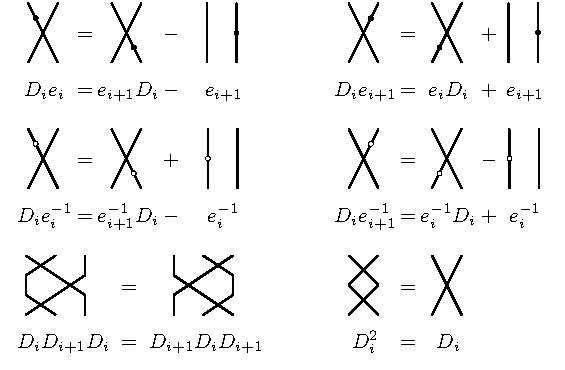
\includegraphics[width=7cm]{strands/relations_1.pdf} 
      \label{fig:relations_1}        
\end{figure}
\end{frame}

\begin{frame}[fragile]{Nontrivial relations II}
\tikz[remember picture, overlay] \node[xshift=12mm, yshift=-2cm, anchor=west] at (current page.north west) {Different color:};

\begin{figure}[ht]
  \vspace{0cm}
    \centering 
    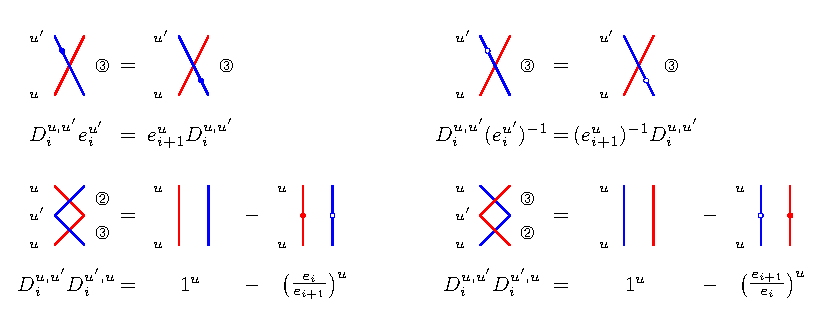
\includegraphics[width=10cm]{strands/relations_2.pdf} 
      \label{fig:relations_2}        
\end{figure}
\end{frame}

\begin{frame}[fragile]{Nontrivial relations III}
\tikz[remember picture, overlay] \node[xshift=12mm, yshift=-2cm, anchor=west] at (current page.north west) {Different color:};
\begin{figure}[ht]
  \vspace{0cm}
    \centering 
    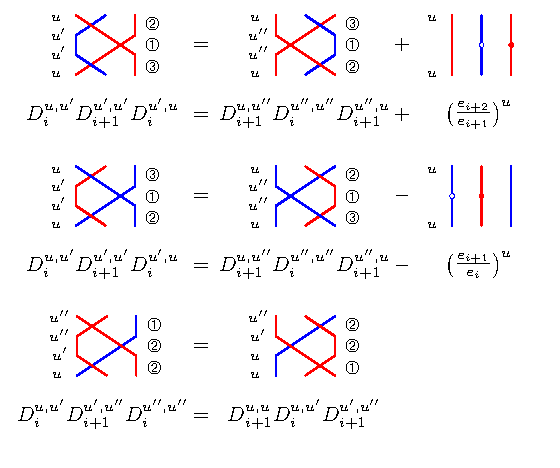
\includegraphics[width=7cm]{strands/relations_3.pdf} 
      \label{fig:relations_3}        
\end{figure}
\end{frame}

\begin{frame}[fragile]{Affine pavings}
内容...
\end{frame}

\begin{frame}[fragile]{Idea of affine pavings}
内容...
\end{frame}

\begin{frame}[fragile]{Outlook}
内容...
\end{frame}
\end{document}